\documentclass{beamer}
\usepackage[utf8]{inputenc}
\usetheme{Madrid}
\usecolortheme{beaver}
\usepackage[style=british]{csquotes}


\usepackage{amsmath}
\usepackage{amsthm}
\usepackage{bm}
\usepackage{graphicx}
\usepackage{accents}

\newcommand{\ubar}[1]{\underaccent{\bar}{#1}}

\newtheorem{prop}{Proposition}



\def\signed #1{{\leavevmode\unskip\nobreak\hfil\penalty50\hskip1em
		\hbox{}\nobreak\hfill #1%
		\parfillskip=0pt \finalhyphendemerits=0 \endgraf}}

\newsavebox\mybox
\newenvironment{aquote}[1]
{\savebox\mybox{#1}\begin{quote}\openautoquote\hspace*{-.7ex}}
	{\unskip\closeautoquote\vspace*{1mm}\signed{\usebox\mybox}\end{quote}}

 
 
%Information to be included in the title page:
\title{An Introduction to Other-Regarding
Preferences With An Application to
Contract Design}
%\subtitle{A Survey}
\author{João Eira}
\institute{FEUC}

\date{2017}
 
 
 
\begin{document}
 
\footnotesize
\begin{frame}[plain]
	\maketitle
	\small
	Supervisor: Prof. Doutor Paulino Teixeira\par\medskip
\end{frame}
\AtBeginSection[]
{
	\begin{frame}{Table of Contents}
		\tableofcontents[currentsection]
	\end{frame}
}
\section{Introduction} 
\begin{frame}
	\frametitle{Introduction}
	\begin{aquote}{F. Y. Edgeworth (1881)}
		The first principle of Economics is that every agent is actuated only by self-interest    
	\end{aquote}

	\begin{aquote}{Adam Smith (1776)}
It is not from the benevolence of the butcher, the brewer, or the baker that we expect our dinner, but from their regard to their own self-interest. We address ourselves not to their humanity but to their self-love, and never talk to them of our own necessities, but of their advantages.
	\end{aquote}
\end{frame}


\begin{frame}
\frametitle{Introduction}
\begin{itemize}
	\item \textbf{Self-regarding preferences:} Preferences are based on states concerning only oneself.
	\begin{itemize}
		\item $U_i \rightarrow U_i\left(y_i\right)$
	\end{itemize}
	\item \textbf{Other-regarding preferences:} Valuations are based in part on what occurs to others.
		\begin{itemize}
		\item $U_i \rightarrow U_i\left(y_i, \vec{\mathbf{y}}_{-i}\right)$
	\end{itemize}
\end{itemize}

\end{frame} 



\section{Selected Games}

\AtBeginSection[]
{
	\begin{frame}{Table of Contents}
		\tableofcontents[currentsection]
	\end{frame}
}

\begin{frame}
	\frametitle{Experimental Games}
	\begin{itemize}
		\item Ultimatum game $\ast$ 
		\item Dictator game
		\item Gift exchange game $\ast$		
		\item Trust game
	\end{itemize}
\end{frame}

\subsection{Ultimatum Game}


\begin{frame}
	\frametitle{Ultimatum Game}
	\textbf{The Ultimatum Game}
	
	A one-shot game between 2 players: A Proposer and a Responder. The Proposer is given an integer amount of tokens, $x$.
	
	\begin{itemize}
		\item Round 1: The Proposer must offer a share $s$ of $x$ to the Responder
		\item Round 2: The Responder decides whether to accept $s$ or not. 
		\begin{itemize}
			\item If the Responder accepts then the Proposer gets $\left(1 - s\right)x$ and the Responder gets $sx$.
			\item If the Responder doesn't accept they both get zero.
		\end{itemize}
	\end{itemize}
	
\end{frame}

\begin{frame}
	\frametitle{Ultimatum Game}
	What happens if both players have self-regarding preferences?

\begin{itemize}
\item Using backwards induction:
\begin{itemize}

\item The Responder has \$0, therefore, he will accept any share.

\item The Proposer, knowing this, will offer the lowest share he can.
\end{itemize}
\end{itemize}

Thus the behavioral prediction for the Ultimatum Game is that the Responder will accept any offer made and the Proposer will offer the lowest amount he can.

\end{frame}

\begin{frame}
	\frametitle{Ultimatum Game}
	How do people actually behave?
	\begin{itemize}
		\item Mean offer is between 30\% to 40\%
		\begin{itemize}
			\item Median offer is between 40\% to 50\%
		\end{itemize}
		\item  Rarely do Proposers offer unfair offers $\left(e.g. s=0.1\right)$or overly generous offers $\left(s>0.5\right)$
		\item  Low offers are often rejected
		\begin{itemize}
			\item Offers below 20\% are rejected half the time
		\end{itemize}
	\end{itemize}

The predictions from self-regarding preferences are therefore not supported by the experimental evidence.

\end{frame}

\subsection{Gift-Exchange Game}

\begin{frame}
	\frametitle{Gift-Exchange Game}
	Two players are each assigned one of two roles: Principal and Agent. 
	\begin{itemize}
	\item The Principal makes a job offer, $\left(w_b,e_n\right)$ to the Agent
	\begin{itemize}
	\item $w_b$ - wage
	\item $e_n$ - \textit{non-binding} effort level
	\end{itemize}
	\item The Agent either accepts or rejects the offer
	\begin{itemize}
	\item If he accepts, he must choose an effort level $e$ to expend
	\begin{itemize}
	\item The Agent incurs a cost $c(e)$ by exerting an effort $e$
	\end{itemize}
	\end{itemize}
	\end{itemize}

\end{frame}

\begin{frame}
\frametitle{Gift-Exchange Game}
What is the self-regarding prediction? 

\begin{itemize}
	\item The Agent will exert the minimum effort level $e_{min}$.
	\item Knowing this, the Principal will offer the lowest $w$ he can.
	\end{itemize}
\end{frame}

\begin{frame}
	\frametitle{Gift-Exchange Game}
	\begin{itemize}
	\item The topic of how fairness concerns affect employment relationships was first broached in (Akerlof, 1982).
	\item He is motivated by (Homans, 1954), where a group of women were found to be exceeding the minimum work requirements by a considerable margin.
	\item Akerlof envisions this relationship as a "gift" exchange mediated by endogenous social norms.
	\begin{itemize}
	\item The works offer a "gift" to the firm in the form of additional effort.
	\item In exchange, the firm offers a "gift" in the form of a wage that is in excess of what they could receive in other jobs.
	\end{itemize}
	\end{itemize}
\end{frame}

\begin{frame}
	\frametitle{Gift-Exchange Game}
	\begin{figure}
	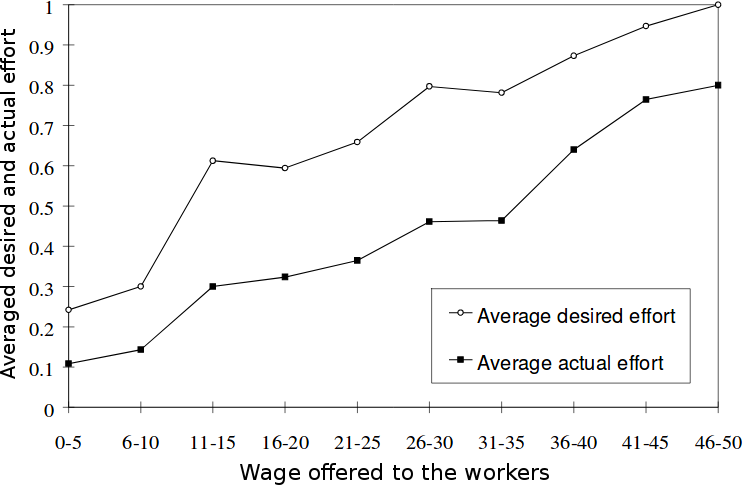
\includegraphics[scale=0.4]{imagens/gift1.png}
	\caption{Source: Fehr and Falk (2002)}
	\end{figure}
\end{frame}

\section{External Validity of Experiments in Economics}

\AtBeginSection[]
{
	\begin{frame}{Table of Contents}
		\tableofcontents[currentsection]
	\end{frame}
}

\begin{frame}
\frametitle{External Validity of Laboratory Experiments}

\textbf{external validity} $\rightarrow$ The ability of of experiments to provide findings that are likely to allow for reliable inferences outside the laboratory

A pernicious problem for the social sciences, in general, and Economics in Particular.

\begin{itemize}
\item If you measure the value of Earth's gravity in a laboratory you need not concern yourself with whether your results will generalize to outside the lab.
\item However, human behavior is highly contextual and so what happens in the laboratory does not necessarily translate into the real world. 
\end{itemize}
\end{frame}

\begin{frame}
\frametitle{External Validity of Laboratory Experiments}

If we want to use the laboratory evidence surveyed previously to argue for the existence of other-regarding inferences then we must first establish that the evidence is reliable for the inference of behavior outside the laboratory. \\~\

Laboratory experiments are often compared with field studies, this last which purports to provide evidence that is more externally valid than laboratory experiments.

\begin{itemize}
\item List (2006) provides an interesting example of this idea. 
\item In his paper he confirms the basic results of the gift exchange game in the laboratory but also employs the gift exchange game in the field.
\item He finds that in the field the behavior of agents, in this case of baseball card dealers, is in line with the predictions of the self-regarding assumption
\end{itemize}

What does this evidence imply for our inference about the existence of other-regarding preferences?

\end{frame}

\begin{frame}
\frametitle{External Validity of Laboratory Experiments}

The answer relies on how much weight we give to one type of evidence versus the other, which will depend on our goals. Colin Camerer distinguishes between the \textit{policy view} and the \textit{scientific view}

\begin{itemize}
\item For the \textit{policy view} the external validity of evidence is of paramount importance and thus field studies performed in the same domain as the policy as obvious advantages.
\item The \textit{scientific view} is concerned with gathering evidence such that our understanding of human behavior is increased, and thus there is no a priori reason for field studies to trump over laboratory experiments.
\end{itemize}

Provided the evidence was properly gathered, there is no hierarchical relationship between field studies and laboratory experiments. Both are tools and the evidence of one set of evidence must be contrasted with the other.

\end{frame}

\begin{frame}
\frametitle{External Validity of Laboratory Experiments}

More specific criticisms of the evidence for other-regarding preferences has appeared however. 

\begin{itemize}
\item \textbf{Experimenter demand effects}
\begin{itemize}
\item Laboratory experiments are highly artificial environments that put subjects under unprecedental scrutinity. Thus subjects might behave in ways that do not reveal their underlying preferences.
\end{itemize}
\item \textbf{Context dependence}:
\begin{itemize}
\item Behavior is context-dependent. It is not clear that laboratory experiments are able to capture this element and control for it.
\end{itemize}
\item \textbf{Self-selection bias}:
\begin{itemize}
\item Laboratory experiments are usually performed with college students as subjects, resulting in multiple experiments run with an homogeneous sample of subjects who might be different than the average human population.
\end{itemize}
\end{itemize}
\end{frame}

\section{Modelling Other-Regarding Preferences}

\AtBeginSection[]
{
	\begin{frame}{Table of Contents}
		\tableofcontents[currentsection]
	\end{frame}
}

\begin{frame}
	\frametitle{The Fehr-Schmidt Model of Inequity Aversion}
	
	Consider $n$ individuals, each with a respective monetary payoff $y_1,y_2,...,y_n$. For any $i$, the Fehr-Schmidt utility function, henceforth FS utility function, is defined as:
	
	\begin{equation}
	\begin{split}
	U_i\left(y_i,\vec{y}_{-i};\alpha_i,\beta_i\right) = y_i & -  \frac{\alpha_i}{n-1} \sum_{j\neq i} \max \left \{ y_j - y_i,0 \right \} \\
	& - \frac{\beta_i}{n-1} \sum_{j\neq i} \max \left \{ y_i - y_j,0 \right \}
	\end{split}
	\end{equation}

where $\alpha_i \geq \beta_i$ and $0 \leq \beta_i <1$.

\end{frame}

\begin{frame}
	\frametitle{The Fehr-Schmidt Model of Inequity Aversion}
\begin{columns}
	\begin{column}{0.5\textwidth}
		\begin{equation*}
			\frac{\alpha_i}{n-1} \sum_{j\neq i} \max \left \{ y_j - y_i,0 \right \} 
		\end{equation*}
		\begin{center}
			Disadvantageous Inequality
		\end{center}
		\begin{center}
		Envy
		\end{center}
	\end{column}
	\begin{column}{0.5\textwidth}  %%<--- here
		\begin{equation*}
\frac{\beta_i}{n-1} \sum_{j\neq i} \max \left \{ y_i - y_j,0 \right \}
\end{equation*}
\begin{center}
	Advantageous Inequality
\end{center}
\begin{center}
	Altruism
\end{center}
	\end{column}
\end{columns}
\end{frame}

\begin{frame}
	\frametitle{The Fehr-Schmidt Model of Inequity Aversion}
	\begin{center}
		\begin{figure}

			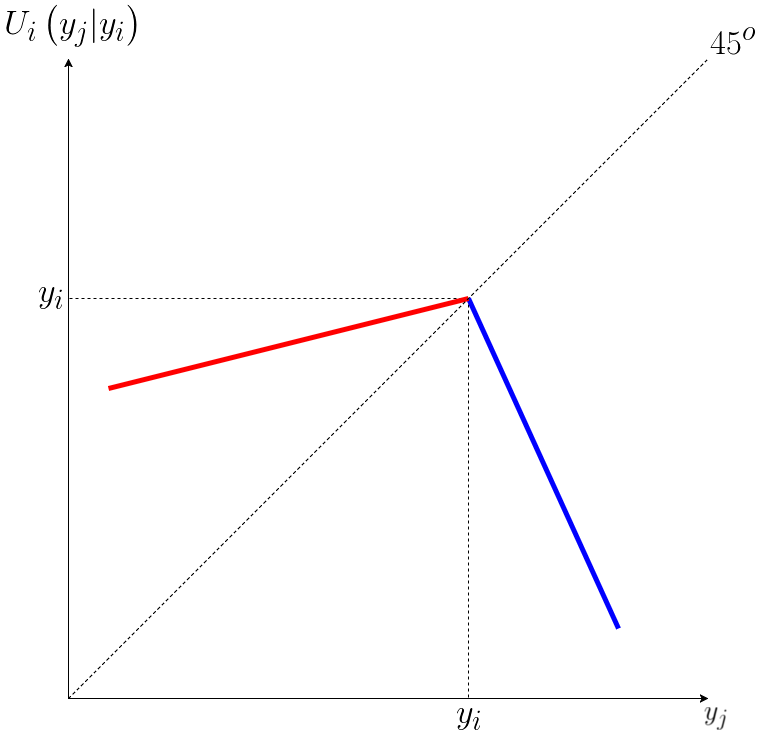
\includegraphics[scale=0.245]{fehrschmidt.png}

		\end{figure}
	\end{center}
	\begin{center}
	\begin{figure}
		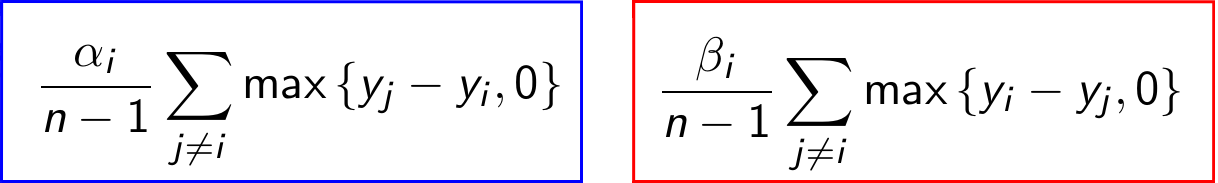
\includegraphics[scale=0.15]{eq.png}
	\end{figure}
\end{center}

	
\end{frame}


\section{Incomplete contracts under other-regarding preferences}

\AtBeginSection[]
{
	\begin{frame}{Table of Contents}
		\tableofcontents[currentsection]
	\end{frame}
}

\begin{frame}
	\frametitle{Incomplete contracts under other-regarding preferences}

	Consider a Principal who wants to hire an Agent. The Agent can expend effort $e \in [\ubar{e}, \bar{e}]$ at a cost $c(e)$ such that $c'>0$ and $c''>0$. The principal wants the Agent to expend $e_{min}$, which he introduces in the contract, but $e_{min}$ is non-binding.

\begin{itemize}
\item The principal might invest in a verification technology that costs $k$
\item The verification technology provides evidence of shirking with probability $p$
\end{itemize}
		
The question is: how should the Principal structure the contract he offers to the Agent such that his goals are best achieved?		
		
		
\end{frame}

\begin{frame}
	\frametitle{Incomplete contracts under other-regarding preferences}
	The three types of contract the Principal has at his disposal are:
\begin{itemize}
	\item \textbf{Incentive contract}: The contract specifies the wage $w$, the contracted effort level $e_c$, and the maximum fine $\bar{f}$.
	\begin{itemize}
	\item $\left(w,e_c,\bar{f}\right)$
	\end{itemize}
	\item \textbf{Trust contract}: The contract specifies the wage $w$ and the contracted effort level $e_c$, which is non-verifiable.
	\begin{itemize}
	\item $\left(w,e_c\right)$
	\end{itemize}
	\item \textbf{Bonus contract}: This contract is similar to the trust contract except if $e>e_c$ the principal might reward the agent with a non-enforceable bonus $b$.
	\begin{itemize}
	\item $\left(w,e_c,b\right)$
	\end{itemize}
\end{itemize}
		
\end{frame}

\begin{frame}
	\frametitle{Incomplete contracts under other-regarding preferences}

\begin{columns}[T] % align columns
\begin{column}{.48\textwidth}
\begin{center}
Incentive Contract

\begin{itemize}
\item The Principal has invested in the verification technology
\item He can induce a positive effort level if the verification technology is potent enough
\item This means that $p\bar{f} \geq c(e^*) - c(\ubar{e})$
\end{itemize}
\end{center}
\end{column}%
\hfill%
\begin{column}{.48\textwidth}

\begin{center}
Bonus Contract


\begin{itemize}
\item $b$ is non-binding
\item The bonus contract is therefore equivalent to the trust contract
\item $b$ Since $e$ is non-binding and non-verifiable, the Agent will exert the lowest possible $e$

\end{itemize}
\end{center}
\end{column}%
\end{columns}

\hfill

\hfill


The prediction is that the Principal will choose the Incentive contract over the Bonus and Trust contracts.		
		
\end{frame}

\begin{frame}
	\frametitle{Incomplete contracts under other-regarding preferences}

	\begin{figure}
	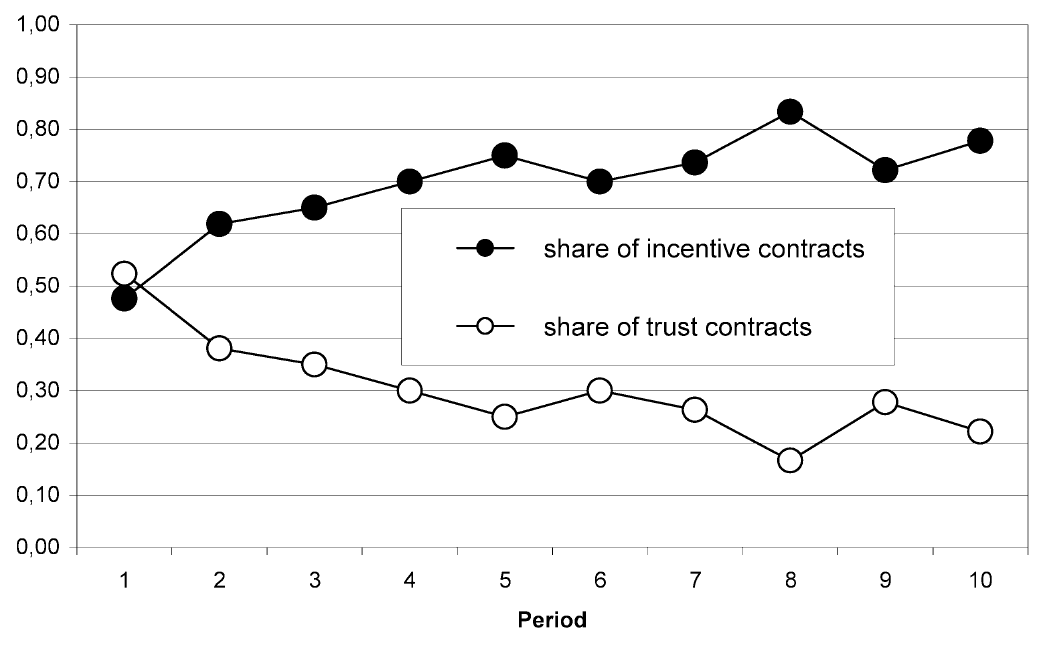
\includegraphics[scale=0.3]{imagens/trustincentive.png}
	\caption{Source: Fehr et al. (2007)}
	\end{figure}
\end{frame}

\begin{frame}
	\frametitle{Incomplete contracts under other-regarding preferences}

	\begin{figure}
	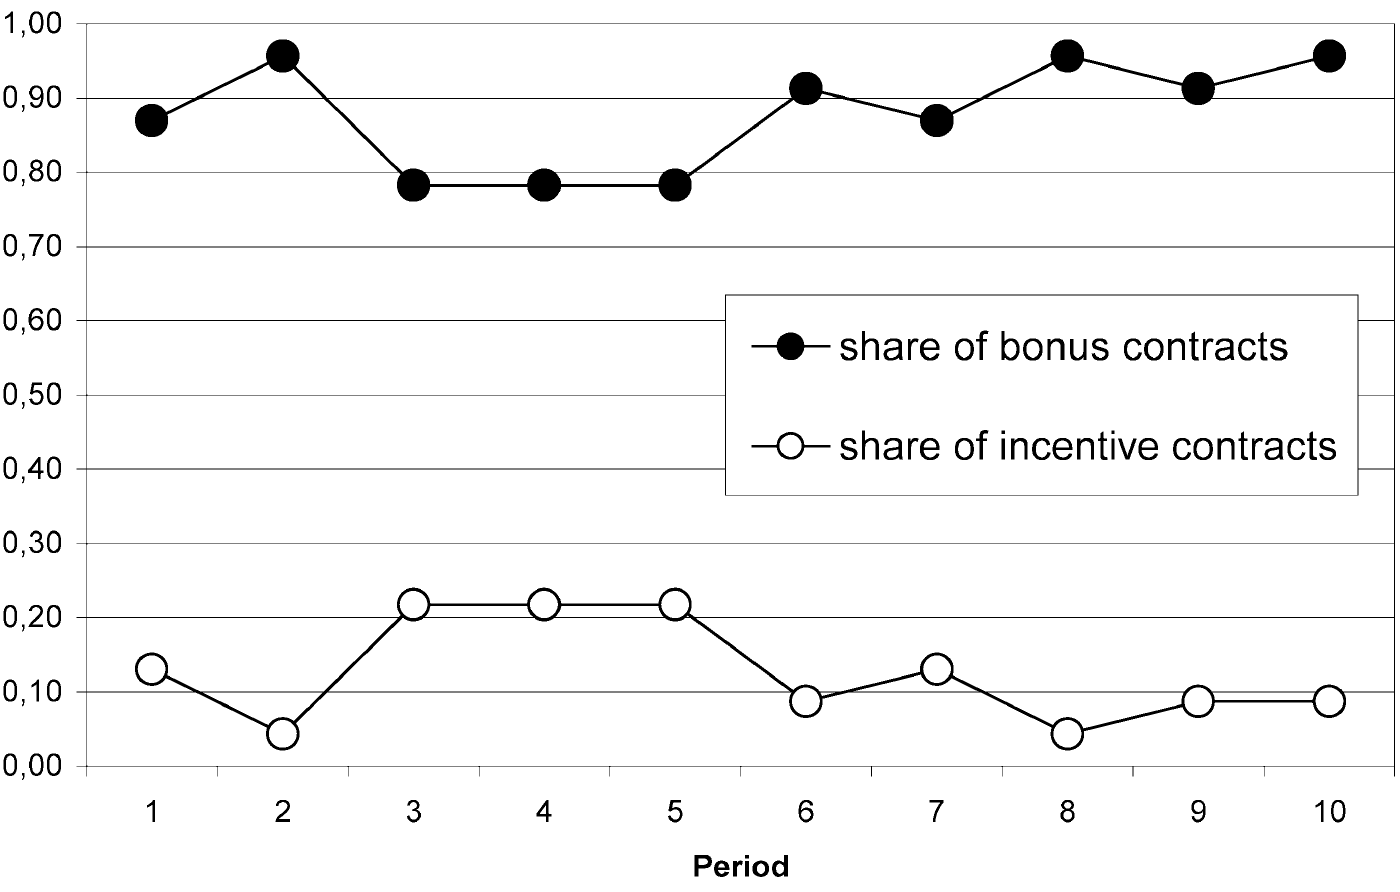
\includegraphics[scale=0.21]{imagens/bonusincentive.png}
	\caption{Source: Fehr et al. (2007)}
	\end{figure}
\end{frame}

\begin{frame}
	\frametitle{Incomplete contracts under other-regarding preferences}
	
For simplicity we will assume that the agent's output is equal to $e$ while the effort cost function is $c(e)=\frac{1}{2}e^2$, where $e\in[0,1]$. \\~\

The utility of a self-regarding agent and principal is given by, respectively

\begin{equation}
	\left\{\begin{matrix}
	u =  & w - \frac{1}{2} e^2 - C_A\\ 
	\pi= & e - w - C_p
	\end{matrix}\right.
\end{equation}

\noindent
where $C_A$ and $C_P$ are whatever other individual costs the agent and principal, respectively, incur by taking part in the relationship.\\~\

We start by describing the expected profits for the principal under
the incentive contract.


\end{frame}

\begin{frame}
	\frametitle{Incomplete contracts under other-regarding preferences}
	\textbf{Incentive contract}\\~\
	
The incentive compatibility constraint of the self-regarding agent is

\begin{equation}
	\left(1-p\right) w + p \left(w-f\right) \leq w - \frac{1}{2}e^2_c
\end{equation}	
	
where we assume $C_A = 0$. This gives us $e_c \leq \sqrt{2pf}$ as the set of effort levels that are incentive compatible. \\~\

Therefore, since $e\in [0,1]$, in an incentive contract where the Principal wishes to maximize profits the optimal contracted effort level is

\begin{equation}\label{eq:min_ei}
	e_I = \min\{1,\sqrt{2pf}\}
\end{equation}
	
\end{frame}

\begin{frame}
	\frametitle{Incomplete contracts under other-regarding preferences}

To maximize profits, the self-interested principal sets a contract $\left(w,e_c\right)$ that maximizes expected profits

\begin{equation}
	E\left(\Pi\right) = \left(1-p\right)\left(e-w-k\right)+p\left(e-w-k+df\right) = e-w-k+pdf
\end{equation}
	

where $d$ is a binary variable dependent on whether $e < e_c$.  \\~\

If $e_c < \sqrt{2pf}$, $d=0$ and $E(\Pi) = e - w - k$. Note that $w \geq \frac{1}{2}e^2_c$. Given that, 

\begin{itemize}
\item If $\sqrt{2pf} \geq 1$ then we have $e_I = 1$ and $w=\frac{1}{2}$. 
\begin{itemize}
\item  $E\left(\Pi\right) = \frac{1}{2} - k$.
\end{itemize}
\item If $\sqrt{2pf} < 1$ then $e_I = \sqrt{2pf}$ and $w=pf$.
\begin{itemize}
\item $E\left(\Pi\right) = \sqrt{2pf} - pf - k$. 
\end{itemize}
\end{itemize}	
	
\end{frame}

\begin{frame}
	\frametitle{Incomplete contracts under other-regarding preferences}
	\textbf{Bonus Contract} \\~\

If $e > e_c$, the bonus will be such that the payoffs of both parties are equaled. 


\begin{equation}
e - w - b = w + b - \frac{1}{2} e^2
\end{equation} 

\noindent
which we solve for $b$ to get

\begin{equation}
	b = \frac{1}{2} e - w + \frac{1}{4}e^2 = b\left(e,w\right)
\end{equation}	
	
\end{frame}

\begin{frame}
	\frametitle{Incomplete contracts under other-regarding preferences}
	

\begin{equation}\label{eq:equalbonus}
	w + b(e,w) - \frac{1}{2}e^2 = e - w - b(e,w)
\end{equation}

Taking the first derivative of (\ref{eq:equalbonus}) in order to $e$ gets us the result that the payoff is maximized at $e^b_F = 1$. 

The other-regarding principal's expected payoff is $E\left(\Pi\right) = e - w - b(e,w)$, which when $e=1$ yields

\begin{equation}
\begin{split}
E\left(\Pi_B\right) & = e - w - \left( \frac{1}{2}e - w + \frac{1}{4}e^2 \right)\\
E\left(\Pi_B\right)& = 1 - w - \frac{1}{2} + w - \frac{1}{4}\\
E\left(\Pi_B\right)& = \frac{1}{4} 
\end{split}
\end{equation}

\end{frame}

\begin{frame}
	\frametitle{Incomplete contracts under other-regarding preferences}
	

So given these options, which contract should the principal prefer? 

\begin{itemize}
\item Under the self-regarding assumption we would expect the incentive contract to dominate over all others. 
\item However, taking into account that principals and agents might have other-regarding preferences, we conclude that the answer depends on a number of parameters. 
\begin{itemize}
\item Suppose that $\sqrt{2pf} > 1$, in which case $E\left(\Pi_I\right) = \frac{1}{2} - k$. For the incentive contract to dominate over the bonus contract it would be needed that $E\left(\Pi_I\right) > E\left(\Pi_B\right)$, that is, $\frac{1}{2} - k > \frac{1}{4}$. This is only true if $ k < \frac{1}{4}$.
\item  For the case where $\sqrt{2pf}<1$ we have that $E\left(\Pi_I\right) = \sqrt{2pf} - pf - k$, which means that the incentive contract dominates over the bonus contract only if $\sqrt{2pf} - pdf - k >\frac{1}{4}$.
\end{itemize}
\end{itemize}
\end{frame}


\section{Conclusion}
\AtBeginSection[]
{
	\begin{frame}{Table of Contents}
		\tableofcontents[currentsection]
	\end{frame}
}

\begin{frame}
	\frametitle{Conclusion}
	\begin{itemize}
		\item As Aristotle put it once, "Man is by nature a social animal."
		\item The self-regarding assumption, while useful, does not account for the full set of documented human behavior
		\item Acknowledging the existence of other-regarding preferences allows economists to extend their studies by taking into account the social aspect of human decision making.
	\end{itemize}
\end{frame}


\begin{frame}
	\frametitle{References}
	\begin{itemize}
		\item Akerlof, G. A. (1982). Labor contracts as partial gift exchange. The quarterly journal of economics, 97(4), 543-569.
		\item Homans, G. C. (1954). The cash posters: A study of a group of working girls. American Sociological Review, 19(6), 724-733.
		\item Fehr, E., \& Falk, A. (2002). Psychological foundations of incentives. European economic review, 46(4-5), 687-724.
		\item Fehr, E., Klein, A., \& Schmidt, K. M. (2007). Fairness and contract design. Econometrica, 75(1), 121-154.
	\end{itemize}
\end{frame}
\end{document}